\documentclass[../main.tex]{subfiles}

% Importing images from another path
\graphicspath{{\subfix{../images/}}}

\begin{document}

The \textbf{Simple Parallel Quicksort} is the first attempted method to
parallelize the quicksort algorithm in a distributed memory environment.
Given a number $P$ of processes, the algorithms first requires to split the
initial array $\mathbf{X}$ into $P$ equally sized\footnote{Plus any eventual remainder distributed in a \textit{round-robin} fashion among the processes.} chunks, $\mathbf{X}^{i}$, of size $n/P$ and then
distribute these sub-arrays among the processes.\\
One of the processes then selects a pivot value $\tau$ and broadcasts it to all the others. This can be easily achieved in MPI~\cite{mpi} thanks to the use of the \cc{MPI\_Bcast} function. Each process can then partition its chunk according to this value forming in this way two local partitions: the \textit{low partition} $\mathbf{X}^{i}_{< \tau}$, with elements smaller than the pivot, and the \textit{high partition} $\mathbf{X}^{i}_{\geq \tau}$, with elements greater or equal to the pivot.\\
Subsequently, any process having rank $i < P/2$ exchanges its high partition
with the low partition of the process with rank $i + P/2$ in a send and receive
operation. Such operation has indeed been implemented in MPI with the \cc{MPI\_Sendrecv} function. This results in processes with rank $i < P/2$  having
only elements smaller than the pivot and processes with rank $i \geq P/2$ having
elements greater or equal than the pivot.\\
The algorithm then proceeds recursively as in the serial version with the lower
rank group of processes working on the \textit{low} part of the array on one hand, while higher rank processes keep sorting the \textit{high} section on the other. In the MPI implemented code this separation is acheved through the use of the \cc{MPI\_Comm\_split} function, which allows to define custom communicators for each subsequent recursive calls.\\
The following pseudocode briefly summarizes the core steps in the MPI implementation:

\begin{codeblock}
\begin{code}{Pseudocode}{MPI Simple Parallel Quicksort}
function MPI_Parallel_qsort($\mathbf{X}^i$, P, comm):
    if P > 1:
        if rank == 0:
            $\tau \leftarrow$ choose_pivot($\mathbf{X}$)
            MPI_Bcast($\tau$, comm)

        $\mathbf{X}^{i}_{< \tau}, \mathbf{X}^{i}_{\geq \tau} \leftarrow$ partition($\mathbf{X}^{i}, \tau$)

        if rank $<$ P/2:
            MPI_Sendrecv($\mathbf{X}^{i}_{\geq \tau}$, $\mathbf{X}^{i+P/2}_{< \tau}$, comm)
        else:
            MPI_Sendrecv($\mathbf{X}^{i}_{< \tau}$, $\mathbf{X}^{i-P/2}_{\geq \tau}$, comm)

        MPI_Comm_split(comm, rank < P/2, low_comm)
        MPI_Comm_split(comm, rank >= P/2, high_comm)

        MPI_Parallel_qsort($\mathbf{X}^i$, P/2, low_comm)
        MPI_Parallel_qsort($\mathbf{X}^i$, P/2, high_comm)
    else:
        $\mathbf{X}_i$ $\leftarrow$ sort($\mathbf{X}_i$)

\end{code}
\caption{Pseudocode for the MPI implemetation of the Simple Parallel Quicksort algorithm.}
\label{code:mpi_simple}
\end{codeblock}

From pseudocode~\ref{code:mpi_simple} it's possible to deduce two observations. First of all, the processes $P$ must be a power of $2$ for the algorithm to work properly, since at each recursive iteration the number of processes is halved. Secondly, the recursion stops when only one process is entering each recursvie call, at which point the local array is sorted using either the serial quicksort ot the \textbf{Task Parallel Quicksort} showed in code~\ref{code:omp_task}. After $\log_2(P)$ recursions, in fact, the largest value in the chunk of the $i^{th}$ process will be smaller than the smallest value in the chunk of the ${ (i+1) }^{th}$ process. The final sorted array can therefore be obtained by simply letting each process sort its partition locally.\\
The average time complexity of this algorithm is $\tilde{\mathcal{O}}(n/P \log n/P)$, but its actual execution is strictly dependent on the choice of the pivot at each recursive call. A bad choice of the pivot might lead to the processes having to work on very differently sized chunks, resulting in a very unbalanced workload.\\
An attempt has also been made to implement a shared memory version of this algorithm using OpenMP~\cite{openmp}.\ This implementation is not as straightforward as its distributed memory counterpart and requires the more complex procedure here described.\\
At the beginning of the recursive call, each thread is assigned an independent portion of the array to be sorted, which, in this case, is a shared variable. One among the threads then picks a pivot and writes its value in a shared variable so that each thread can parallely partition its portion in place. Since in OpenMP there's no direct way to perform message passing, nor to exchange the partitions between threads, the next step assumes the form of a global rearrangement of the elements in the array according to a shared \cc{indexes} array. Such operation requires to know in advance where the elements of each thread's partition will be placed in the final array. In order to find these positions, each thread first writes the count of elements in its low partition on a reserved location of a shared array $\mathbf{L}$. The same happens for the high partitions in an array $\mathbf{H}$. The prefix sum is then performed on these arrays so that

\begin{itemize}
    \item the $j^{th}$ element in the low partition of the $i^{th}$ thread will end up in position \\$L[i] + j$ from the start of the initial array\footnote{The first element of both the $\mathbf{L}$ and $\mathbf{H}$ arrays is set to $0$ to account for the final position of the first elements in each partition.};
    \item the $j^{th}$ element of the high partition of the $i^{th}$ thread will end up in position \\$L[P] + H[i] + j$ from the start of original array\footnote{Where $P$ here is also the total number of threads.}.
\end{itemize}

Therefore, each thread can independently compute the final positions for the elements in its partitions and write these in the corresponding locations of the shared \cc{indexes} array. This whole procedure is schematically depicted in figure~\ref{fig:prefix_sum}.\\
Before entering the next recursive call, one among the threads takes the job of serially rearranging the elements of the array according to the so computed \cc{indexes} array. Unfortunately, this last step requires a sequential execution in order to avoid possible data races or other types of undefined behaviors. This indeed constitutes the major bottleneck of this implementation.\\

\begin{figure}[bh]
    \centering

    % Tikz Image (better)
    \begin{tikzpicture}

        % x-axis for reference
        % \draw[line width=0.2, -Stealth] (0, 1.5) -- (10, 1.5);
        % % numbers on x-axis
        % \foreach \i in {0, 1, ..., 10} {
        %     \node at (\i, 1.75) {\i};
        % }

        % Define the colors
        \definecolor{lightblue}{HTML}{0080ff}

        % 1D array rectangle
        \draw[line width=0.2] (0, 0) rectangle (10, 0.5);

        % Highlight the first cell of first chunk in yellow
        \draw[fill=yellow, opacity=0.5] (0, 0) rectangle (0.5, 0.5);
        \node at (0.25, -0.25) {pivot $\tau$};

        % Fill the array with the numbers
        \foreach \value [count=\i] in {7, 13, 18, 2, 17, 1, 14, 20, 6, 10,
                                       15, 9, 3, 16, 19, 4, 11, 12, 5, 8} {
            \node at (\i*0.5-0.25, 0.25) {\value};
            \draw[line width=0.1] (\i*0.5, 0) -- (\i*0.5, 0.5);
        }

        % Separation of the chunks
        \draw[line width=0.5, dashed, color=gray] (0, 0.5) -- (0, 1);
        \node at (1, 0.75) {$P_0$};
        \draw[line width=0.5, dashed, color=gray] (2, 0.5) -- (2, 1);
        \node at (3, 0.75) {$P_1$};
        \draw[line width=0.5, dashed, color=gray] (2, 0.5) -- (2, 1);
        \node at (5, 0.75) {$P_2$};
        \draw[line width=0.5, dashed, color=gray] (4, 0.5) -- (4, 1);
        \node at (7, 0.75) {$P_3$};
        \draw[line width=0.5, dashed, color=gray] (6, 0.5) -- (6, 1);
        \node at (9, 0.75) {$P_4$};
        \draw[line width=0.5, dashed, color=gray] (8, 0.5) -- (8, 1);
        \draw[line width=0.5, dashed, color=gray] (10, 0.5) -- (10, 1);

        \node[anchor=west] at (10, 0.25) {Input $\mathbf{X}$};

        % Array after partitioning
        \draw[line width=0.2] (0, -1) rectangle (10, -0.5);
        \draw[fill=lightblue, opacity=0.3] (0, -1) rectangle (0.5, -0.5);
        \draw[fill=red, opacity=0.3] (0.5, -1) rectangle (2, -0.5);
        \draw[fill=lightblue, opacity=0.3] (2, -1) rectangle (2.5, -0.5);
        \draw[fill=red, opacity=0.3] (2.5, -1) rectangle (4, -0.5);
        \draw[fill=lightblue, opacity=0.3] (4, -1) rectangle (4.5, -0.5);
        \draw[fill=red, opacity=0.3] (4.5, -1) rectangle (6, -0.5);
        \draw[fill=lightblue, opacity=0.3] (6, -1) rectangle (7, -0.5);
        \draw[fill=red, opacity=0.3] (7, -1) rectangle (8, -0.5);
        \draw[fill=lightblue, opacity=0.3] (8, -1) rectangle (8.5, -0.5);
        \draw[fill=red, opacity=0.3] (8.5, -1) rectangle (10, -0.5);
        \foreach \value [count=\i] in {2,7,18,13,1,17,14,20,6,10,15,9,3,4,19,16,5,12,11,8} {
            \node at (\i*0.5-0.25, -0.75) {\value};
            \draw[line width=0.1] (\i*0.5, -1) -- (\i*0.5, -0.5);
        }
        \draw[line width=0.5, dashed, color=gray] (2, -0.5) -- (2, 0);
        \draw[line width=0.5, dashed, color=gray] (2, -0.5) -- (2, 0);
        \draw[line width=0.5, dashed, color=gray] (4, -0.5) -- (4, 0);
        \draw[line width=0.5, dashed, color=gray] (6, -0.5) -- (6, 0);
        \draw[line width=0.5, dashed, color=gray] (8, -0.5) -- (8, 0);
        \draw[line width=0.5, dashed, color=gray] (10, -0.5) -- (10, 0);
        \node[anchor=west] at (10, -0.75) {Partitioning};

        % Prefix sum arrays
        \node[anchor=east] at (0.5, -2.25) {$\mathbf{L}$};
        \draw[line width=0.2] (0.5, -2.5) rectangle (3.5, -2);
        \foreach \value [count=\i] in {0,1,1,1,2,1} {
            \node at (\i*0.5+0.25, -2.25) {\value};
            \draw[line width=0.1] (\i*0.5, -2.5) -- (\i*0.5, -2);
        }

        \node[anchor=west] at (9.5, -2.25) {$\mathbf{H}$};
        \draw[line width=0.2] (6.5, -2.5) rectangle (9.5, -2);
        \foreach \value [count=\i] in {0,3,3,3,2,3} {
            \node at (\i*0.5+6.25, -2.25) {\value};
            \draw[line width=0.1] (\i*0.5+6, -2.5) -- (\i*0.5+6, -2);
        }

        % Dashed arrows from partitions to prefix sum arrays
        \draw[line width=0.5, dashed, color=lightblue, 
              opacity=0.5, -Stealth] (0.25, -1.05) -- (1.25, -1.95);
        \draw[line width=0.5, dashed, color=lightblue, 
              opacity=0.5, -Stealth] (2.25, -1.05) -- (1.75, -1.95);
        \draw[line width=0.5, dashed, color=lightblue, 
              opacity=0.5, -Stealth] (4.25, -1.05) -- (2.25, -1.95);
        \draw[line width=0.5, dashed, color=lightblue, 
              opacity=0.5, -Stealth] (6.5, -1.05) -- (2.75, -1.95);
        \draw[line width=0.5, dashed, color=lightblue, 
              opacity=0.5, -Stealth] (8.25, -1.05) -- (3.25, -1.95);
        \draw[line width=0.5, dashed, color=red, 
              opacity=0.5, -Stealth] (1.25, -1.05) -- (7.25, -1.95);
        \draw[line width=0.5, dashed, color=red, 
              opacity=0.5, -Stealth] (3.25, -1.05) -- (7.75, -1.95);
        \draw[line width=0.5, dashed, color=red, 
              opacity=0.5, -Stealth] (5.25, -1.05) -- (8.25, -1.95);
        \draw[line width=0.5, dashed, color=red, 
              opacity=0.5, -Stealth] (7.5, -1.05) -- (8.75, -1.95);
        \draw[line width=0.5, dashed, color=red, 
              opacity=0.5, -Stealth] (9.25, -1.05) -- (9.25, -1.95);

        \node[anchor=west] at (1.1, -2.75) {prefix sum};
        \node[anchor=west] at (7.1, -2.75) {prefix sum};
        \draw[line width=0.5, color=gray, -Stealth] (0.75, -2.55) -- (0.75, -2.95);
        \draw[line width=0.5, color=gray, -Stealth] (3.25, -2.55) -- (3.25, -2.95);
        \draw[line width=0.5, color=gray, -Stealth] (6.75, -2.55) -- (6.75, -2.95);
        \draw[line width=0.5, color=gray, -Stealth] (9.25, -2.55) -- (9.25, -2.95);

        % Prefix sum arrays n2
        \node[anchor=east] at (0.5, -3.25) {$\mathbf{L}$};
        \draw[line width=0.2] (0.5, -3.5) rectangle (3.5, -3);
        \foreach \value [count=\i] in {0,1,2,3,5,6} {
            \node at (\i*0.5+0.25, -3.25) {\value};
            \draw[line width=0.1] (\i*0.5, -3.5) -- (\i*0.5, -3);
        }

        \node[anchor=west] at (9.5, -3.25) {$\mathbf{H}$};
        \draw[line width=0.2] (6.5, -3.5) rectangle (9.5, -3);
        \foreach \value [count=\i] in {0,3,6,9,11,14} {
            \node at (\i*0.5+6.25, -3.25) {\value};
            \draw[line width=0.1] (\i*0.5+6, -3.5) -- (\i*0.5+6, -3);
        }

        % Final array
        \draw[line width=0.2] (0, -5) rectangle (10, -4.5);
        \draw[fill=lightblue, opacity=0.3] (0, -5) rectangle (3, -4.5);
        \draw[fill=red, opacity=0.3] (3, -5) rectangle (10, -4.5);
        \foreach \value [count=\i] in {2,1,6,3,4,5,7,18,13,17,14,20,10,15,9,19,16,12,11,8} {
            \node at (\i*0.5-0.25, -4.75) {\value};
            \draw[line width=0.1] (\i*0.5, -5) -- (\i*0.5, -4.5);
        }
        \foreach \value [count=\i] in {0,1,2,3,4,5,6,7,8,9,10,11,12,13,14,15,16,17,18,19} {
            \node[color=gray] at (\i*0.5-0.25, -5.25) {\small\value};
        }
        \node[anchor=west] at (10, -4.75) {Rearranged $\mathbf{X}$};

        % Connecting lines
        \draw[line width=0.5] (6.75, -1.05) -- (6.75, -1.5);
        \draw[line width=0.5] (6.75, -1.5) -- (4.5, -1.5);
        \draw[line width=0.5] (4.5, -1.5) -- (4.5, -4);
        \draw[line width=0.2, color=lightblue, fill=white] (4, -2.75) rectangle (5, -3.25);
        \node[anchor=center] at (4.5, -3) {$j=1$};
        \draw[line width=0.5, -Stealth] (2.25, -3.55) -- (2.25, -4.45);
        \node[anchor=east] at (2.25, -4) {$L[3] + 1 = 4$};
        \draw[fill=lightblue, opacity=0.15] (2.05, -4) circle (0.2);
        \draw[fill=lightblue, opacity=0.15] (2.25, -5.28) circle (0.2);
        \draw[line width=0.5] (2.25, -4) -- (4.5, -4);

        \draw[line width=0.5] (5.75, -1.05) -- (5.75, -4);
        \draw[line width=0.2, color=red, fill=white] (5.25, -2.75) rectangle (6.25, -2.25);
        \node[anchor=center] at (5.75, -2.5) {$j=2$};
        \draw[line width=0.5] (7.75, -3.55) -- (7.75, -4);
        \draw[line width=0.5] (5.75, -4) -- (7.75, -4);
        \draw[line width=0.5, -Stealth] (7.25, -4) -- (7.25, -4.45);
        \node[anchor=west] at (7.75, -4) {$L[5] + H[2] + 2 = 14$};
        \draw[fill=red, opacity=0.15] (10.86, -4) circle (0.2);
        \draw[fill=red, opacity=0.15] (7.25, -5.28) circle (0.2);



    \end{tikzpicture}

    % PNG Image (Commented)
    % 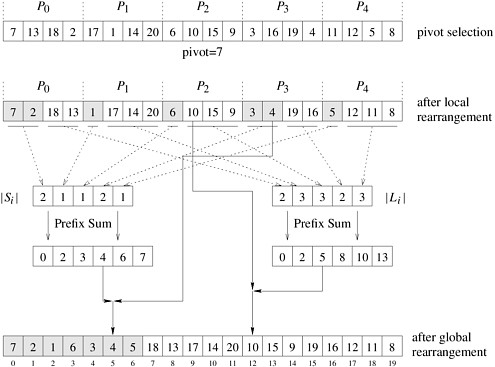
\includegraphics[width=10cm]{prefix_sum.jpg}

    \caption{Rearrangement of partitions in shared memory using the prefix sum and $P=5$ threads~\cite{intropar}. The pivot value is highligted in yellow, low partitions $\mathbf{X}^i_{<}$ are in blue and high partitions $\mathbf{X}^i_{\geq}$ are in red. Note that thread numbering is zero-based so the first thread will be identified by $i=0$.} 
    \label{fig:prefix_sum}
\end{figure}

\end{document}